\section{Граничные обратные задачи и задачи с данными Коши}\label{sec:rev}

\subsection{Граничная обратная задача}\label{subsec:rev}
\begin{frame}
    \frametitle{Граничная обратная задача}
    Модель имеет следующий вид
    \begin{wrapfigure}{r}{0.3\textwidth}
        \centering{\includegraphics[width=1\linewidth]{omega_1}}
%        \caption*{$\Gamma \coloneqq \partial \Omega =\overline{\Gamma}_0 \cup \overline{\Gamma}_1 \cup \overline{\Gamma}_2$}
    \end{wrapfigure}
    \begin{gather}
        \label{eq:2_1:initial}
        - a \Delta \theta + b \kappa_a(\theta ^ 3 | \theta | - \varphi) = 0, \\
        - \alpha \Delta \varphi + \kappa_a (\varphi - \theta ^3 | \theta |) = 0,
    \end{gather}
    \begin{equation}
        \label{eq:2_1:initial-boundary}
        \begin{aligned}
            \Gamma &: \; a \partial_n \theta + \beta (\theta - \theta _b) = 0, \\
            \Gamma_0 \cup \Gamma_2 &: \; \alpha \partial_n \varphi
            + \gamma(\varphi - \theta_b ^4 ) = 0, \\
            \Gamma_1 &: \; \alpha \partial_n \varphi + u(\varphi - \theta_b ^4 ) = 0. \\
        \end{aligned}
    \end{equation}
    $\Gamma_0, \Gamma_1, \Gamma_2$ не имеют пересечений.

    Функции $\gamma, \theta_b, \beta$ известны.
    \textit{Неизвестная функция $u$ характеризует отражающие свойства участка границы $\Gamma_1$}.
    Предполагается, что $0 < u_1 \leq u \leq u_2$.

    \textbf{Обратная задача} заключается в отыскании тройки $\theta, \varphi, u$
    по дополнительному условию $\theta|_{\Gamma_2} = \theta_0$.

    \textbf{Экстремальная задача} заключается в минимизации функционала
    \begin{equation}
        \label{eq:2_1:quality}
        J(\theta) = \frac{1}{2} \int_{\Gamma_2} (\theta - \theta_0)^2 d\Gamma
    \end{equation}
    на решениях краевой задачи~\eqref{eq:2_1:initial}--\eqref{eq:2_1:initial-boundary}.
\end{frame}
\note{
    Первая из рассматриваемых задач формулируется следующим образом:
    дана некая область омега,
    на части её границы неизвестен параметр среды $u$, характеризирующий отражающие свойства границы.
    Сам параметр выражается как $(\frac{\varepsilon}{2(2-\varepsilon)})$, где $\varepsilon$ меняется в диапазоне от 0 до 1,
    как следствие на сам параметр накладывается ограничение, такое что $u \in [0, 0.5]$.

    Степень черноты не зависит от направления и определяется формулой
    $\varepsilon_\nu(x) = \frac{I_{\nu,\text{исп}}(x)}{I_{b\nu}(T(x))}$, где
    $I_{\nu,\text{исп}}(x)$ -- интенсивность излучения, испускаемого
    поверхностью при температуре $T(x)$~\cite[53]{Ozisik1976}.
    Требуется отыскать тройку: температурное поле,
    поле излучения и неизвестный параметр
    по дополнительной информации о температуре на границе.
    Вопрос о корректности сформулированной обратной задачи является открытым
    (как её решать тоже вопрос открытый).
    Предлагается заменить обратную задачу на задачу
    оптимального управления, которая состоит в
    минимизации функционала~\eqref{eq:2_1:quality}.
    Решение данной экстремальной задачи называется квазирешением обратной задачи.
    Для нахождения квазирешения был разработан оптимизационный численный метод.

    Постоянные $a$ (температуропроводность $м^2/сек$), $b$(коэфициент радиационного переноса) и
    $\alpha$ (Эффективный коэффициентом оптического взаимодействия)
    определяются следующим образом:
    \[
        a = \frac{k}{\rho c_v},\quad b = \frac{4\sigma n^2 T_{\max}^3}{\rho c_v},
        \quad \alpha=\frac{1}{3\kappa - A \kappa_s},
    \]
    где $k$ -- теплопроводность $(Вт/(м \cdot К)=Дж/(м \cdot с \cdot К))$, $c_v$ -- удельная теплоемкость,
    $\rho$ -- плотность,
%    $\sigma$ -- постоянная Стефана-Больцмана $(5.67 \cdot 10^{−8} Вт/(m^2 \cdot K^4))$,
    $n$ -- показатель преломления,
%    $T_{\max}$ -- максимальная температура в ненормализованной модели,
%    $\kappa = \kappa_s + \kappa_a$ -- коэффициент
%    полного взаимодействия,
%    $\kappa_s$ -- коэффициент рассеяния, $\kappa_a$ -- коэффициент поглощения.
}


\begin{frame}
    \frametitle{Нахождение квазирешения обратной задачи}
    \begin{gather}
        A_1 \theta + b \kappa_a (| \theta | \theta^3 - \varphi) =
        f, A_2 \varphi + \kappa_a (\varphi - |\theta|\theta^3) + F(\varphi, u) = g.
        \label{eq:2_1:weakOperational}\\
        J(\theta) = \frac{1}{2} \int_{\Gamma_2} (\theta - \theta_0)^2 d\Gamma,
        \label{eq:2_1:qualityOperational}\\
        A_1 p_1 + 4 |\hat{\theta}|^3 \kappa_a(b p_1 - p_2) = f_c,
        \;\; (f_c,v) = - \int_{\Gamma_2} (\hat{\theta} - \theta_0) v d\Gamma,
        \label{eq:2_1:theorem_2_eq1}\\
        A_2 p_2 + \kappa_a (p_2-b p_1) = g_c(p_2, \hat{u}),
        \;(g_c(p_2, \hat{u}), v) = -\int_{\Gamma_1} \hat{u} p_2 v d\Gamma,
        \label{eq:2_1:theorem_2_eq2}\\
        \int_{\Gamma_1} p_2 (\hat{\varphi} - \theta_b^4)(u-w) d\Gamma
        \leq 0 \quad \forall w \in U_{ad}. \label{eq:2_1:theorem_2_eq3}
    \end{gather}
    \textbf{Алгоритм градиентного спуска с проекцией}
    \begin{enumerate}
        \item Выбор шага $\lambda$, числа итераций $N$, управления $u_0 \in U_{ad}$
        -- пространство допустимых управлений.
        \item для $k \leftarrow 0,1,2, \ldots, N$ выполнить:
        \begin{itemize}
            \item Для $u_{k}$, вычислить $y_k = \{\theta_k, \varphi_k\}$ из~\eqref{eq:2_1:weakOperational}.
            \item Вычислить значение $J(\theta_k)$ из уравнения~\eqref{eq:2_1:quality}.
            \item Рассчитать $p_k=\{p_{1k},p_{2k}\}$
            из~\eqref{eq:2_1:theorem_2_eq1}--\eqref{eq:2_1:theorem_2_eq2},
            \item Пересчитать управление
            $u_{k+1} = P_{ad}\left[ u_k - \lambda (\varphi_k - \theta_b^4)p_{2k} \right]$.
        \end{itemize}
    \end{enumerate}
\end{frame}
\note{
    Предложенный в работе алгоритм поиска квазирешения обратной задачи основан
    на выведенных условиях оптимальности
    (доказано, что квазирешение должно
    удовлетворять~\eqref{eq:2_1:weakOperational}--\eqref{eq:2_1:theorem_2_eq2}),
    куда входят сопряженные функции для температуры $p_1$ и излучения $p_2$,
    а также связь между сопряженным состоянием и искомым граничным управлением.
    Для компактной записи краевых задач, используется современная операторная форма.
    Система~\eqref{eq:2_1:weakOperational} является операторной записью краевой задачи,
    где $A_{1,2}$ описывают диффузионные члены модели, остальные моделируют граничные условия.
    Уравнения~\eqref{eq:2_1:theorem_2_eq1}--\eqref{eq:2_1:theorem_2_eq2}
    это сопряженная система,
    а вариационное неравенство~\eqref{eq:2_1:theorem_2_eq3}
    устанавливает связь с оптимальным управлением.

    Приведём алгоритм градиентного спуска с проекцией.
    Обратим внимание, что оператор проекции нужен
    из-за начальных ограничений на функцию управления
    (вызванных физичностью параметра, например).

    Отметим, что в силу невыпуклости экстремальной задачи градиентные алгоритмы не обладают
    свойством глобальной сходимости, что служит основой для их критики, зачастую заслуженной.

    Однако свойства диффузионных моделей сложного теплообмена представленные в диссертации
    и правильный выбор шага градиентного метода обеспечивают сходимость для
    рассматриваемых задач.
    Следующие примеры этот факт демонстрируют.
}

\begin{frame}
    \frametitle{Модель управления температурным полем через граничный параметр}
    Положим $\Omega = \{(x,y), 0 \leq x,y \leq 1\}$, $l = 1$ см.
    Граница $\partial\Omega$:
    \[
        \begin{aligned}
            \Gamma_0 & = \{x=\{0,1\}, y \in [0,1]\} \\
            \Gamma_1 & = \{x\in [0,1], y=0\}
            - \text{участок с неизвестными отр. свойствами}, \\
            \Gamma_2 & = \{x \in [0,1], y=1\} - \text{участок наблюдения}.
        \end{aligned}
    \]
    Будем также далее считать, что $a = 0.006[\text{см}^2/\text{c}]$,
    $b=0.025[\text{см}/\text{с}]$, $\beta = 0.00005[\text{см}/\text{с}]$,
    $\kappa=1[\text{см}^{-1}]$, $\kappa_s = 0$, $A = 0$, $\gamma = 0.3$.
    Температуру на границе $\Omega$ положим равной $\theta_b = (x^2+y^2)/3$.

    При указанных параметрах для первого эксперимента выберем следующее тестовое
    значение функции $u$:
    \begin{equation*}
        u(x)=
        \begin{cases}
            0.01, & \text{если } x \le 0.5, \\
            0.5, & \text{если } x > 0.5,
        \end{cases}
    \end{equation*}
    и для второго эксперимента:
    $u(x)=0.49x+0.01$.
\end{frame}
\note{
    Положим параметры среды, соответствующие стеклу и зададим тестовую функцию управления
    как показано на слайде.
    Пластинка, у которого боковые стороны "обычные", верхняя грань - участок наблюдения,
    нижняя грань - участок под "контролем".
}


\begin{frame}
    \frametitle{Модель управления температурным полем через граничные параметр}
    \centering
    \includegraphics[width=0.42\linewidth]{dvmg368/3}
    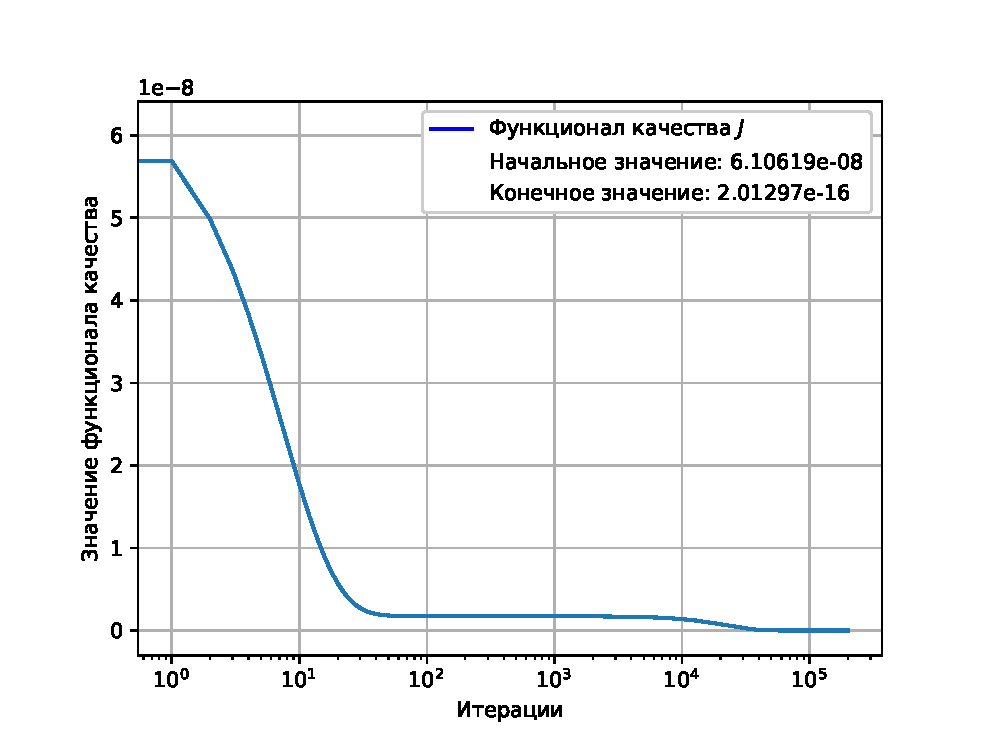
\includegraphics[width=0.42\linewidth]{dvmg368/4}
    \includegraphics[width=0.42\linewidth]{dvmg368/1}
    \includegraphics[width=0.42\linewidth]{dvmg368/2}
\end{frame}
\note{
    Интересный эффект "среднего значения". Большое количество итераций.
    Обратить внимание на функционал качества.
    Для получения представленных результатов, использовался разработанный мной комплекс программ,
    включающий решение прямой задачи, сопряженной системы и алгоритм градиентного спуска.
}

\subsection{Обратная задача с условиями типа Коши}\label{subsec:rev_koshi}
\begin{frame}
    \frametitle{Задача без краевых условий для интенсивности излучения}
    \textbf{Краевая задача:}
    \begin{equation}
        \label{eq:2_2:eq1}
        - a \Delta \theta + b \kappa_a(\theta ^ 3 | \theta | - \varphi) = 0,  \quad
        - \alpha \Delta \varphi + \kappa_a (\varphi - \theta ^3 | \theta |) = 0,
    \end{equation}
    На $\Gamma$ известно температурное поле и тепловой поток:
    \begin{equation}
        \label{eq:2_2:bc2} \theta = \theta_b, \quad \partial_n\theta = q_b.
    \end{equation}
    Заменяем на <<искусственные>> краевые условия
    \begin{equation}
        \label{eq:2_2:bc3}
        a(\partial_n\theta+\theta) = r,\;\;
        \alpha(\partial_n\varphi+\varphi) = u \text{ на }\Gamma.
    \end{equation}
    Функция $r(x),\, x\in\Gamma$ является заданной, функция $u(x),\, x\in\Gamma$
    описывающая излучающие свойства участка границы, неизвестна.
    Получаем \textbf{обратную задачу}.

    \textbf{Экстремальная задача} заключается в отыскании тройки
    $\{\theta_\lambda,\varphi_\lambda,u_\lambda\}$ такой, что
    \begin{equation}
        \label{eq:2_2:cost}
        J_\lambda(\theta, u) = \frac{1}{2}\int\limits_\Gamma (\theta - \theta_b)^2 d\Gamma
        + \frac{\lambda}{2}\int\limits_\Gamma u^2 d\Gamma \rightarrow\inf
    \end{equation}
    на решениях краевой задачи, функция $u(x) x \in \Gamma$ играет роль управления.

    \begin{itemize}
        \item $(j) \;\; a,b,\alpha,\kappa_a, \lambda ={\textrm Const}> 0,$
        \item $(jj) \;\, \theta_b, \,q_b \in U,\;\; r=a(\theta_b+q_b)$.
    \end{itemize}
    \begin{theorem}[2.3]
        \label{th:2_2:1}
        Пусть выполняются условия $(j), (jj)$.
        Тогда существует решение экстремальной задачи.
    \end{theorem}
\end{frame}
\note{
    23. Не задано $\varphi$!
    В основе разработанного алгоритма решения лежит анализ экстремальной задачи.

    Строго обосновано существование решения экстр задачи.
    Кроме того, и это принципиально важно, показана сходимость решений экстремальных задач
    к решению задачи~\eqref{eq:2_2:eq1}--\eqref{eq:2_2:eq2}
    без краевых условий для интенс излучения при $\lambda$ стремящемся к 0.
}
\begin{frame}
    \frametitle{Пример 1}
    \textbf{Задача $CP$.} Найти тройку $\{\theta, \varphi, u \} \in V \times V \times U$
    такую, что
    \begin{equation}
        \label{eq:2_2:cp}
        J_\lambda(\theta, u) \equiv \frac{1}{2}\|\theta -\theta_b\|^2_\Gamma
        + \frac{\lambda}{2}\|u\|^2_\Gamma \rightarrow \inf,\;\; F(\theta, \varphi, u)=0.
    \end{equation}
    Для обозначенных параметров рассчитаем функции $\theta$, $\varphi$ из решения граничной задачи
    и положим $\theta_b = \theta|_\Gamma$.
    Нормальная производная $\partial_n \theta = q_b = r / a - \theta_b$.

    Применяя алгоритм градиентного спуска найдем решение задачи $CP$.
    \begin{figure}[h!t]
        \begin{minipage}[b][][b]{0.49\linewidth}
            \centering
            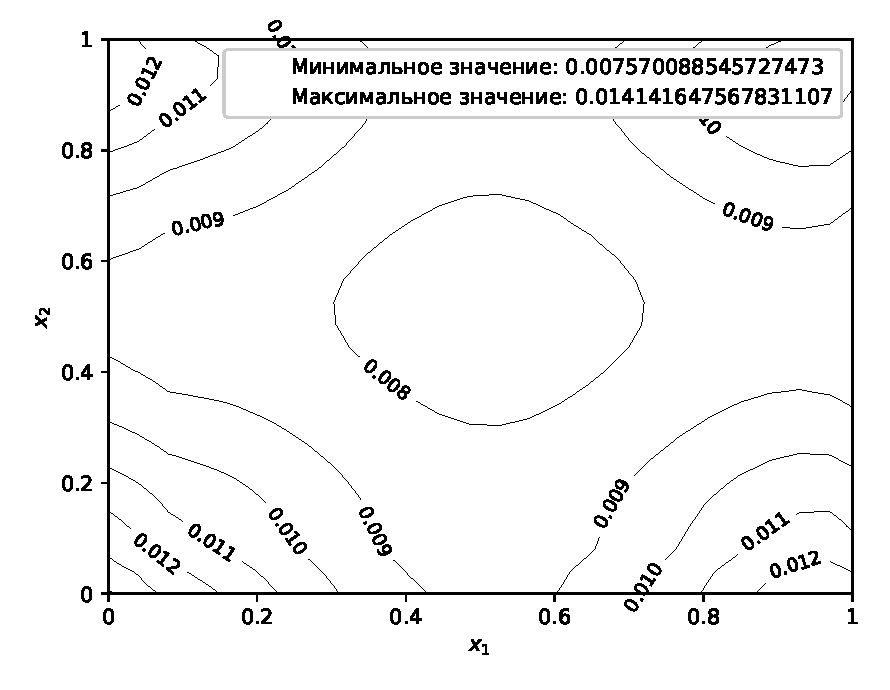
\includegraphics[width=1\linewidth]{jvm-2020/exp1/theta_n_diff_iso}
            \\ а) $|\partial_n\theta_\lambda-q_b|/|q_b|$
        \end{minipage}
        \hfill
        \begin{minipage}[b][][b]{0.49\linewidth}
            \centering
            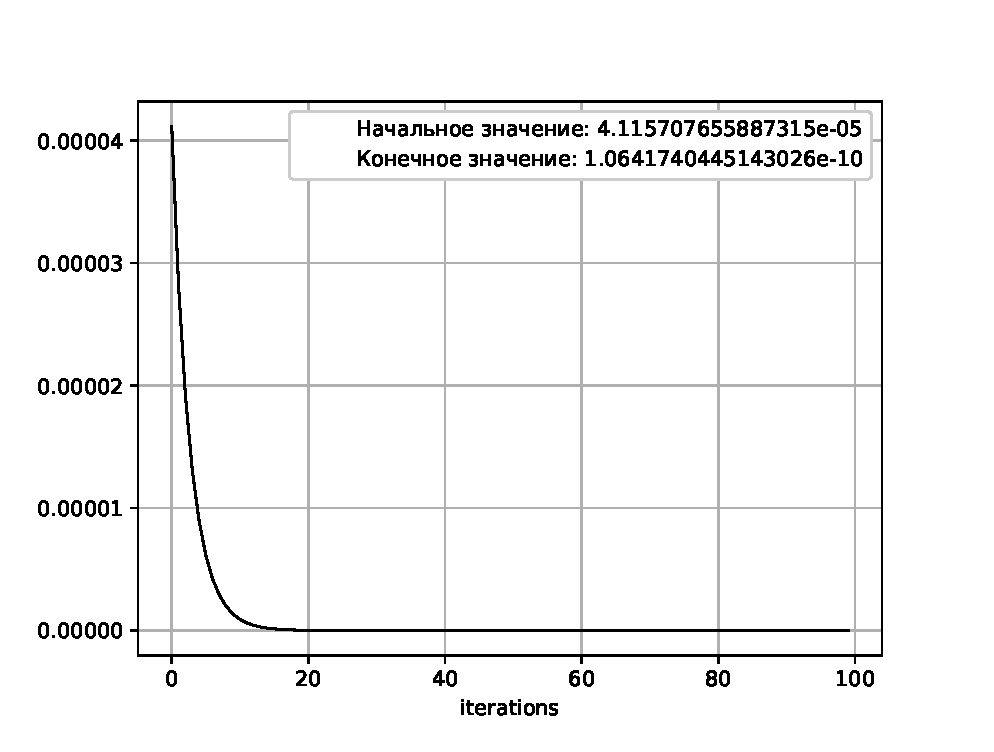
\includegraphics[width=1\linewidth]{jvm-2020/exp1/quality}
            \\ б) Значение функционала качества
        \end{minipage}
        \label{fig:4_4:0}
    \end{figure}
\end{frame}
\note{
    Обратите внимание на малость функционала качества.
    Сравним с тем, что получилось -- довольно близко, но не идеально.
    Уменьшение параметра регуляризации повышает точность решения,
    но и увеличивает вычислительные затраты.
}

\begin{frame}
    \frametitle{Пример 2}
    Зададим функции $\theta_{b}, q_{b}$ в краевом условии~\eqref{eq:2_2:bc2}
    следующим образом:
    \[
        \theta_{b}=0.1 z+0.3, \quad q_{b}=
        \begin{cases}
            0.11, & \text { если } z=1, \\
            0, & \text { если } 0<z<1, \\
            -0.15, & \text { если } z=0.
        \end{cases}
    \]

    В данном примере оптимальное управление $u$ в качестве тестового не задается.

    \begin{figure}[h!t]
        \begin{minipage}[b][][b]{0.49\linewidth}
            \centering
            \includegraphics[width=0.9\linewidth]{jvm-2020/dvmg/3a}
            \\ а) Изменение функционала в зависимости от числа итераций
        \end{minipage}
        \hfill
        \begin{minipage}[b][][b]{0.49\linewidth}
            \centering
            \includegraphics[width=1\linewidth]{jvm-2020/dvmg/2b}
            \\ б) Оптимальное управление
        \end{minipage}
        \label{fig:4_4:3}
    \end{figure}

\end{frame}
\note{
    "Честный" эксперимент - используем то, что полагается в исходной задаче.
    Функционал качества (его динамика) позволяет предположить аналогичный порядок
    близости (с предыдущим примером)
    точного и аппроксимированного решений.
    Обратите внимание на линейность $\theta_b$ по оси $z$.
}


\begin{frame}
    \frametitle{Квазистационарная модель с данными Коши}
    \textbf{Начально-краевая задача:}
    \begin{equation}
        \label{eq:2_3:1}
        \begin{split}
            & \frac{\partial \theta}{\partial t} - a \Delta \theta
            + b \kappa_{a} \left(|\theta| \theta^{3}-\varphi\right) = 0,\\
            & - \alpha \Delta \varphi
            + \kappa_{a} \left(\varphi-|\theta| \theta^{3}\right) = 0,
            \quad x \in \Omega, \quad 0 < t < T;
        \end{split}
    \end{equation}
    \begin{align}
        a \left(\partial_{n} \theta+\theta\right)=r,
        & \quad \alpha\left(\partial_{n} \varphi
                          + \varphi\right) = u \text { на } \Gamma;  \label{eq:2_3:2}\\
        & \left.\theta\right|_{t=0} = \theta_{0}. \label{eq:2_3:3}
    \end{align}


    \textbf{Экстремальная задача} состоит в том, чтобы найти тройку
    $\left\{\theta_{\lambda}, \varphi_{\lambda}, u_{\lambda}\right\}$ такую, что
    \begin{equation}
        \label{eq:2_3:4}
        J_{\lambda}(\theta, u)=\frac{1}{2} \int_{0}^{T}
        \int_{\Gamma}\left(\theta-\theta_{b}\right)^{2} d \Gamma d t+\frac{\lambda}{2}
        \int_{0}^{T} \int_{\Gamma} u^{2} d \Gamma d t \rightarrow \inf
    \end{equation}
    на решениях задачи~\eqref{eq:2_3:1}--\eqref{eq:2_3:3}.
    \begin{itemize}
        \item $(k)\; a, b, \alpha, \kappa_{a}, \lambda=$ Const $>0$,
        \item $(kk)\; \theta_{b}, q_{b} \in U, r=a\left(\theta_{b}+q_{b}\right)
        \in L^{5}(\Sigma), \; \theta_{0} \in L^{5}(\Omega)$.
    \end{itemize}


    \begin{theorem}[2.8]
        \label{th:2_3:3}
        Пусть выполняются условия $(k), (kk)$ и существует решение
        $\theta, \varphi \in$ $L^{2}\left(0, T ; H^{2}(\Omega) \right)$
        задачи~\eqref{eq:2_3:1}--\eqref{eq:2_3:3}.
        Если $\left\{\theta_{\lambda}, \varphi_{\lambda}, u_{\lambda}\right\}$
        — решение задачи оптимального управления при $\lambda>0$, то при $\lambda\rightarrow+0$
        \[
            \begin{gathered}
                \theta_{\lambda} \rightarrow \theta \text { слабо в } L^{2}(0, T ; V),
                \text { сильно в } L^{2}(Q), \\
                \varphi_{\lambda} \rightarrow \varphi \text { слабо в } L^{2}(0, T ; V).
            \end{gathered}
        \]
    \end{theorem}
\end{frame}
\note{
    \begin{itemize}
        \item Рассмотрим квазистационарный вариант постановки задачи, которые учитывают изменения температурного поля во времени.
        \item Результат о корректности (разр.+ед.) модели в ходе диссертации удалось обобщить на квазистационарный случай.
        \item Также доказана сходимость предложенного оптимизационного метода к решениям исходной задачи.
        \item Начально-краевая задача решается явной схемой.\ Для теоретического обоснования устойчивости
        использовался критерий Куранта-Фридрихса-Леви + численные эксперименты.
        \item Укрупнение шага по времени в десять раз меняет итоговое решения
        в шестом знаке после запятой -- большой запас устойчивости явной схемы.
    \end{itemize}

    CFL: $\Delta t \leq C (\Delta x)^2 / a \rightarrow$ зависимость от шага сетки.
    Суть, что передача тепла не должна "перепрыгивать" узел за шаг по времени. \\
    число Куранта: $\nu =\frac{\Delta t}{(\Delta x)^2)} \text{ характеристическая скорость диффузии } \leq C$,
    $С$ - константа, зависящая от схемы (обычно 0.5 или 1 для простых схем).
}

\begin{frame}
    Область $\Omega \times(-L, L)$,
    где $\Omega=$ $\left\{x=\left(x_{1}, x_{2}\right): 0<x_{1,2}<d\right\}$.

    Определим параметры:
    $d=1(\text{м})$, $a=9.21 \times 10^{-5}(\text{м}^{2} / \text{с})$,
    $b=0.19(\text{м} / \text{с})$, $\alpha=0.0333(\text{м})$,
    $\kappa_{a}=1\left(\text{м}^{-1}\right)$, $T = 1(\text{c})$.
    \begin{figure}[h!t]
        \begin{minipage}[b][][b]{0.49\linewidth}
            \centering
            \includegraphics[width=1\linewidth]{paper03/1} \\ а) Поле температуры,
            полученное в статье *
        \end{minipage}
        \hfill
        \begin{minipage}[b][][b]{0.49\linewidth}
            \centering
            \includegraphics[width=1\linewidth]{paper03/2} \\
            б) Поле температуры, полученное предложенным алгоритмом
        \end{minipage}
        \label{fig:4_3:1}
    \end{figure}
    \tiny{* A. Y. Chebotarev, A. E. Kovtanyuk и N. D. Botkin. — \textit{«Problem of
    radiation heat exchange with boundary conditions of the Cauchy type»}. —
    Communications in Nonlinear Science and Numerical Simulation 75 (2019), с. 262—269.}
\end{frame}
\note{
    \begin{itemize}
        \item Приведём сравнение результатов работы предложенного в дисс.\ алгоритма и метода решения коллег из Мюнхена.
        \item Николай Боткин (слева) использовал разработанную в TUM программу, использующую эрмитов прямоугольный (конформный) элемент Богнера-Фокса-Шмидта.
        \item Фактически ему пришлось решать краевую задачу для нелинейного уравнения 4 порядка.
        \item Результаты применения предложенного нами алгоритма справа.
        \item Параметры задачи были взяты из статьи наших коллег.
        \item наш алгоритм проще (сложнее ошибиться в реализации) + теоретич.\ обоснован, не использует различную экзотику.
        \item Лишён артефактов не свойственных для диффузионных моделей.
    \end{itemize}
    Среда — перегретый водяной пар (90-95\%) с примесью воздуха 5-10\%) и сажей ($10^{-6}-10^{-7}$),
    обеспечивающей оптическую толщину порядка единицы на масштабе 1м. \\
    \textit{Реальные применения: 1) Сушилки на перегретом паре с рециркуляцией дымовых газов.
    2) Паровые котлы и теплообменники с рециркуляцией топочных газов (биомасса, мазут);
    3) Системы утилизации тепла во влажно-газовых средах (целлюлозно-бумажная, химическая промышленность).}
}

\begin{frame}
    \frametitle{Стац.\ задача с условиями Коши для температуры на части границы}
    \begin{wrapfigure}{r}{0.4\textwidth}
        \centering{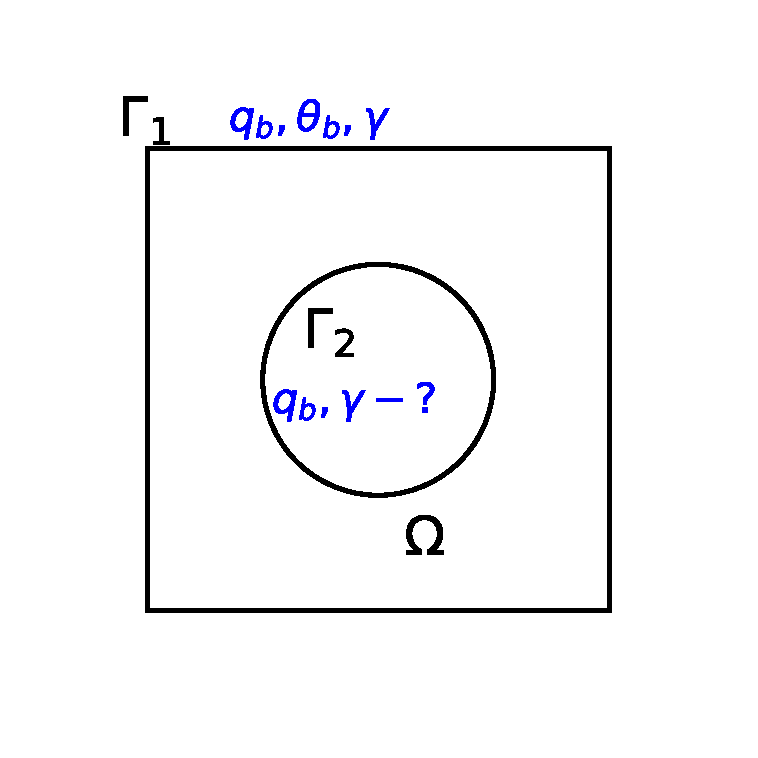
\includegraphics[width=1\linewidth]{omega-circle}}
%        \caption*{$\Gamma \coloneqq \partial \Omega =\overline{\Gamma}_0 \cup \overline{\Gamma}_1 \cup \overline{\Gamma}_2$}
    \end{wrapfigure}
    Рассмотрим область $\Omega$ с границей $\Gamma=\partial\Omega$.
    \begin{gather}
        \label{eq:2_4:eq1}
        - a\Delta\theta + b\kappa_a(\theta^4 - \varphi) = 0,   \\
        -\alpha \Delta \varphi + \kappa_a(\varphi- \theta^4) = 0.
    \end{gather}
    $\Gamma \coloneqq \partial \Omega = \overline{\Gamma}_1 \cup \overline{\Gamma}_2$
    так, что $\Gamma_1 \cap \Gamma_2 = \emptyset$.
    На всей границе $\Gamma$ задается тепловой поток $q_b$,
    \begin{equation}
        \label{eq:2_4:bc1}
        a \partial_n \theta = q_b, \quad x \in \Gamma.
    \end{equation}
    Для задания краевого условия для интенсивности излучения требуется знать функцию $\gamma$.
    В случае, если эта функция неизвестна на части границы $\Gamma_2$,
    краевое условие для интенсивности излучения на $\Gamma_2$ не ставится, а в качестве условия
    переопределения на $\Gamma_1$, в дополнение к условию на
    $\varphi$, задается температурное поле $\theta_b$,
    \begin{equation}
        \label{eq:2_4:bc2}
        \alpha\partial_n\varphi + \gamma (\varphi - \theta_{\text{out}} ^4 ) = 0,\;
        \theta=\theta_b\quad \text{ на } \Gamma_1.
    \end{equation}.

\end{frame}
\note{
    \begin{itemize}
        \item Наиболее сложная с теоретической точки зрения постановка.
        \item На всей границе известен поток, а параметр из граничного условия
        для $\varphi$ неизвестен.
        Мы дополняем ``доступный'' участок информацией о температуре: $\theta_b$.
        \item Нет известных теоретических результатов о корректности
        \item Однако, предложенный оптимизационный метод полностью обоснован, и лежит в основе соотв.\ программного комплекса.
        \item Доказана разрешимость, условия оптимальности, сходимость регуляризованных решений к решению обратной задачи при $\lambda \to 0$.
        \item Это значит, что если решение существует (берём некоторую реальную физическую задачу), то предложенный алгоритм найдёт решение.
    \end{itemize}
    \vspace{2em}
    \textit{Теплозащитные экраны (ТЗЭ) спускаемых аппаратов обычно делают из частично прозрачных
    материалов: углеродные композиты, керамические теплозащитны плиты и так далее.
    Эти материалы частично прозрачны в видимом и ближнем ИК-диапазоне,
        особенно при высоких температурах.}
    \\ \textit{Обратные задачи и данные Коши:} \\
    \textit{На внешней поверхности ТЗЭ температура и тепловой поток измеряются
    датчиками (термопары, пирометры), но на внутренней поверхности
        (интерфейс с конструкцией) данные отсутствуют или недоступны.} \\
    \textit{Оптимальное управление:} \\
    \textit{Можно оптимизировать толщину/состав покрытия,
        чтобы минимизировать перегрев конструкции при заданных внешних условиях.}
}


\begin{frame}
    \textbf{Численное моделирование.}
    Рассмотрим трёхмерный случай:

    Куб $S = \{(x, y, z), 0 \leq x,y,z \leq 1~\text{см.}\}$ с
    круговой полостью $R$ с центром $b_0 =\{0.5, 0.5, 0.5\}$
    $R = \{r, \| r - b_0 \| \leq 0.15~\text{см.} \}$.

    Рассматриваемая область $\Omega = S \setminus R$.
    $\Gamma \equiv \partial \Omega = \partial C \cup \partial B$, при этом
    $ \Gamma_2 = \partial R, \Gamma_1 = \partial S \setminus \Gamma_2$.
    Параметры среды соответствуют стеклу. \\
    Граничные данные $q_b$ и $\theta_b$ положим равными
    $
    q_b =
    \begin{cases}
        -0.2, & x \in \Gamma_1, \, z \in \{0, 1\}, \\
        0,   & x \in \Gamma_1, \, z \in (0, 1), \\
        0.2, & x \in \Gamma_2.
    \end{cases}
    $
    \begin{figure}[h!t]
        \begin{minipage}[b][][b]{0.49\linewidth}
            \centering
            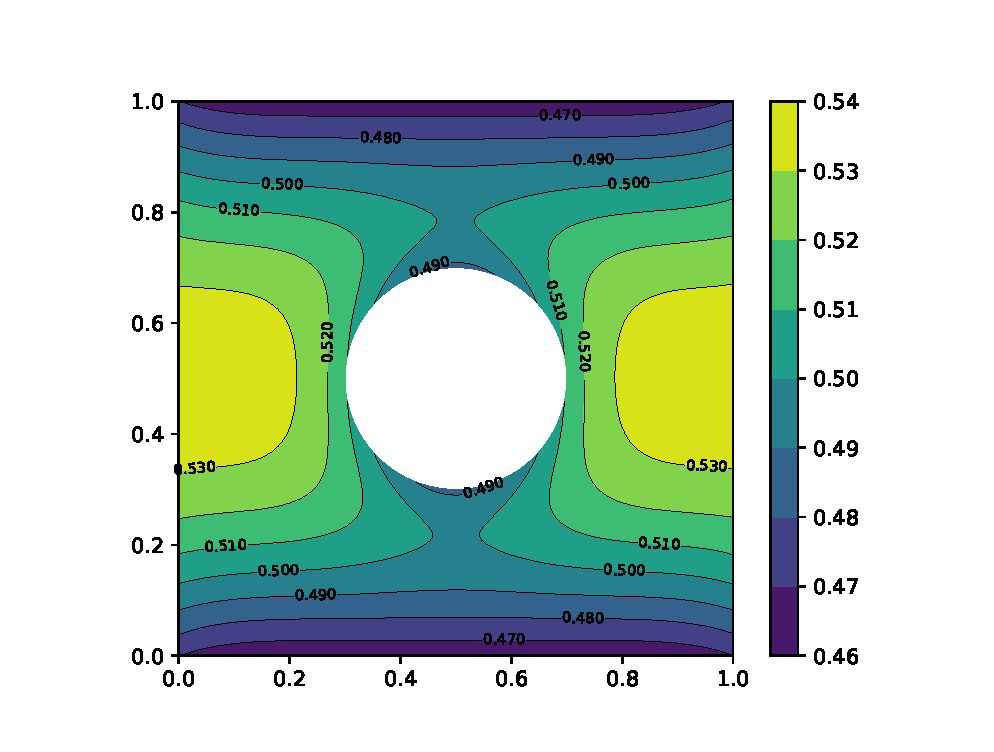
\includegraphics[width=1\linewidth]{theta_endf}
            \\ а) $\theta$
        \end{minipage}
        \hfill
        \begin{minipage}[b][][b]{0.49\linewidth}
            \centering
            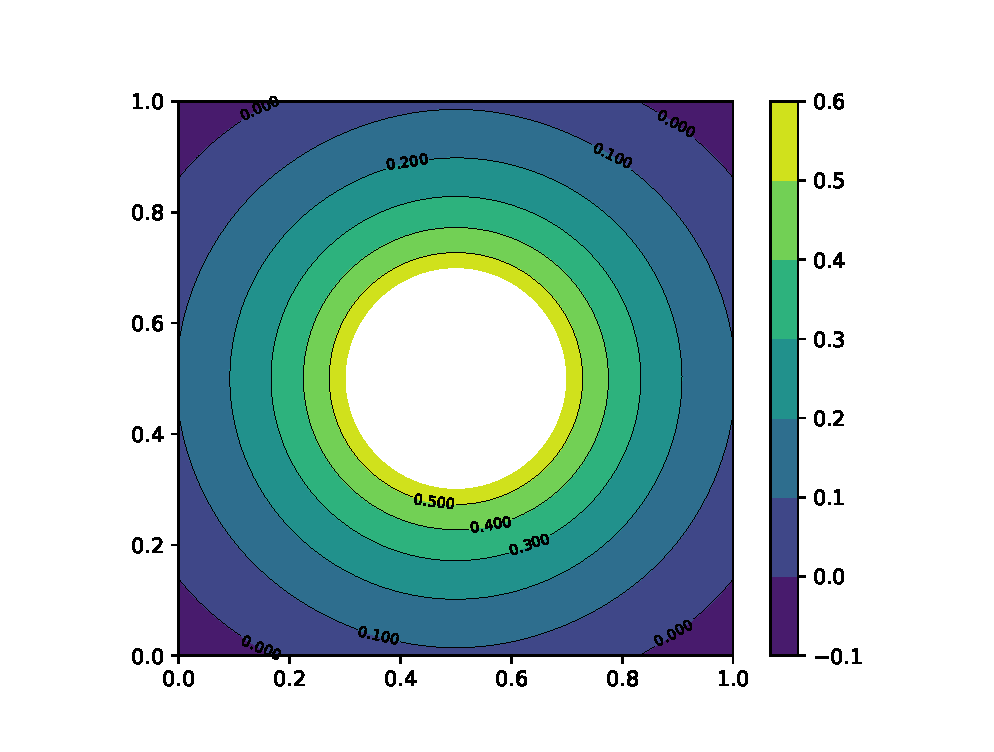
\includegraphics[width=1\linewidth]{phi_endf}
            \\ б) $\varphi$
        \end{minipage}
        \label{fig:4_4:6}
    \end{figure}
    Начальное значение функционала качества $0.045$
    после тридцати итераций становится равным $6.2\cdot10^{-5}$.
\end{frame}
\note{
    \begin{itemize}
        \item 3D-геометрия: куб внутренней круговой полостью (центр в (0.5, 0.5, 0.5)).
        \item  $\varphi$: концентрические круги — типичное диффузионное распределение излучения.
        \item  Поля гладкие, без артефактов — подтверждает устойчивость и корректность метода в 3D.
        \item  $J$ упал с $0.045$ до $6.2e-5$ за 30 итераций — высокая эффективность алгоритма.
    \end{itemize}
}


\begin{frame}
    \frametitle{Исследование устойчивости решений обратных задач с данными Коши}
    Положим $a\partial_n \theta = q_b +\varepsilon \psi$, где $\psi = \psi(x)$, $x \in \Gamma_1$ функция возмущения.

    Полученное решение задачи~\eqref{eq:2_4:eq1},~\eqref{eq:2_4:bc2} обозначим за $\theta^{\varepsilon}$.
    $\theta$ будет соответствовать случаю $\varepsilon = 0$.

    Область $\Omega$ -- квадрат с единичной стороной, $\Gamma_1$ соответствует стороне $y = 1$.

    Положим $\theta_b = (x + y) / 2$ и $q_b = a / 2$, $\varepsilon \in [-0.1, 0.1]$,
    вычислим $L^2$ норму отклонения возмущенного поля.
    \begin{figure}[h!t]
        \begin{minipage}[b][][b]{0.4\linewidth}
            \centering
            \includegraphics[width=1\linewidth]{additional/2/deps_1}\\ а) $\psi = 1,$
        \end{minipage}
        \hfill
        \begin{minipage}[b][][b]{0.4\linewidth}
            \centering
            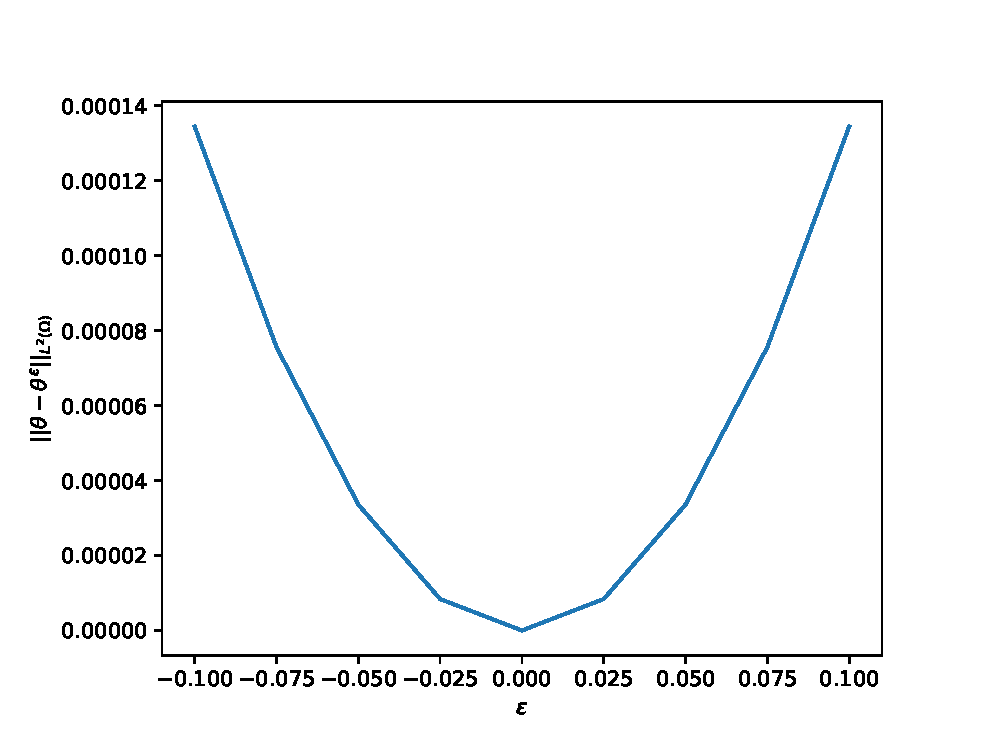
\includegraphics[width=1\linewidth]{additional/2/eps_sin} \\ б) $\psi = \sin (100 * \pi x)$.
        \end{minipage}
        \caption{$||\theta^\varepsilon - \theta||^2_{L^2(\Omega)}$}
        \label{fig:4_4:vareps}
    \end{figure}
    Численные эксперименты демонстрируют
    устойчивость решения относительно изменений теплового потока.
\end{frame}
\note{
    \begin{itemize}
        \item Классическая проблема: эллиптические уравнения с данными Коши неустойчивы
        (пример Адамара: малые изменения потока $\rightarrow$ большие изменения решения).
        \item Для нашей модели с радиационно-кондуктивным обменом теоретическая устойчивость остаётся открытой.
        \item На первом этапе проблему устойчивости проверили численно: в условие Неймана добавлен шум c интенсивностью $\varepsilon$.
        \item Рассмотрены два типа возмущений:
        \begin{itemize}
            \item константное $\varPsi = 1$,
            \item быстро осциллирующее $\varPsi= sin(100 \pi x$).
        \end{itemize}
        \item Вычислена $L^2$-норма отклонения $\theta^\varepsilon$ от $\theta$ (чистое решение при $\varepsilon = 0$).
        \item Результаты: линейная зависимость отклонения от $\varepsilon$ в обоих случаях.
        \item Вывод: модель демонстрирует практическую устойчивость к возмущениям потока (ошибкам замеров).
        \item Полученные данные позволяют выдвинуть гипотезу об устойчивости рассматриваемой модели,
        которую наша группа планирует обосновать теоретически.
    \end{itemize}}


\begin{frame}
    \frametitle{Квазилинейная модель c фазовыми ограничениями}
    \begin{wrapfigure}{r}{0.34\textwidth}
        \centering{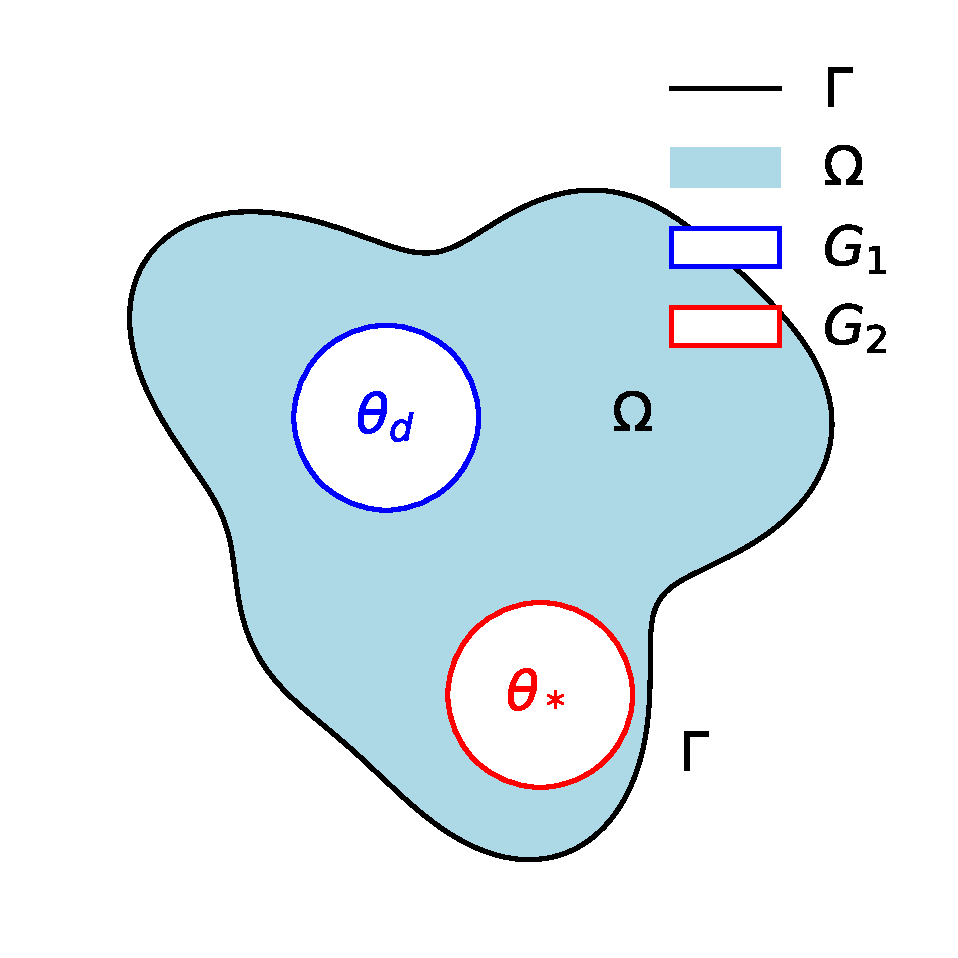
\includegraphics[width=1\linewidth]{omega-g1-g2}}
%        \caption*{$\Gamma \coloneqq \partial \Omega =\overline{\Gamma}_0 \cup \overline{\Gamma}_1 \cup \overline{\Gamma}_2$}
    \end{wrapfigure}

    \textbf{Задача оптимального управления $P$} \\
    заключается в минимизации функционала
    \[ J(\theta)=\int_{0}^{T} \int_{G_{1}}\left(\theta-\theta_{d}\right)^{2} dx dt \rightarrow \inf \]
    на решениях начально-краевой задачи:
    \begin{equation}
        \label{eq:3_2:1}
        \begin{gathered}
            \sigma \partial \theta / \partial t-\operatorname{div}(k(\theta)
            \nabla \theta)-\beta \varphi=u_{1} \chi \\
            -\operatorname{div}(\alpha \nabla \varphi)+\beta \varphi=u_{2}
            \chi, \quad x \in \Omega, \quad t \in(0, T),
        \end{gathered}
    \end{equation}
    \begin{equation}
        \label{eq:3_2:2}
        \theta=\left.0\right|_{\Gamma},
        \quad \alpha \partial_{n} \varphi
        +\left.2^{-1} \varphi\right|_{\Gamma}=0,
        \left.\quad \theta\right|_{t=0}=\theta_{0}.
    \end{equation}
    При этом учитываются ограничения:
    \[ u_{1,2} \geq 0, \quad u_{1}+u_{2} \leq P, \left.\quad \theta\right|_{G_{2}} \leq \theta_{*} \]

    \textbf{Задача со штрафом $P_{\varepsilon}$}.
    $J_{\varepsilon}(\theta) \rightarrow \inf$, где
    \[
        \begin{aligned}
            & J_{\varepsilon}(\theta)=\int_{0}^{T}
            \int_{G_{1}}\left(\theta-\theta_{d}\right)^{2} dx dt
            +\frac{1}{\varepsilon} \int_{0}^{T}
            \int_{G_{2}} F(\theta) d x d t, \\
            & \sigma \theta^{\prime}+A(\theta)=u,
            \quad \theta(0)=\theta_{0}, \quad u \in U_{a d},\\
            &F(\theta)=
            \begin{cases}
                0, & \text { если } \theta \leq \theta_{*} \\
                \left(\theta-\theta_{*}\right)^{2},
                & \text { если } \theta>\theta_{*}.
            \end{cases}
        \end{aligned}
    \]

\end{frame}
\note{
    \begin{itemize}
        \item В том случае, если важно учесть изменения параметров среды от температуры используются квазилинейные модели.
        \item Сама модель представлена уравнением~\eqref{eq:3_2:1}.
        Параметр теплопроводности зависит от температуры.
        \item Такие модели возникают при моделировании эндовенозной лазерной коагуляции.
        \item Сама задача формулируется следующим образом: дана область, в ней две подобласти.
        \item В синей хотим температурное поле $\theta_d$ в красной мы не хотим превышения $\theta_*$.
        \item В диссертации доказана разрешимость исходной задачи, а также оптимизационный метод штрафа, для которого тоже
        доказана разрешимость, а также его сходимость к начальной постановке.
        \item Сама идея метода штрафа заключается в том, что мы добавляем ``штрафное'' слагаемое в функционал качества.
        Слагаемое равно нулю, если температура меньше критической, и быстро растёт, если больше.
    \end{itemize}
    $P$ – максимальная мощность источника,
    $\alpha$ – коэффициент диффузии фотонов,
    $Hi$ есть характеристическая функция той части среды, в которой он расположен, деленная на его объём.
    $\beta$ – коэффициент поглощения, $k(\theta)$ является коэффициентом теплопроводности,
    $\sigma$ является произведением удельной теплоемкости и плотности среды,
    $u_1$ описывает мощность источника тепла, $u_2$ – мощность источника теплового излучения.

    Главная проблема здесь-наличие ограничения на температуру в области $G_2$.
    Для ее преодоления рассматривается задача со штрафом.
    Нарушение указанного ограничения штрафуется ростом функционала при малых значениях $\epsilon$.
    Обоснована сходимость предложенного штрафного алгоритма к решению задачи
    с ограничениями на температуру при $\epsilon\to+0$.
}
\begin{frame}
    \textbf{Условия разрешимости и сходимость решений при $\varepsilon \rightarrow +0$}
    \begin{itemize}
        \item $(c1)\; \sigma_{0} \leq \sigma \leq \sigma_{1}, \quad|\partial \sigma / \partial t| \leq \sigma_{2}$
        \item $(c2)\; k_{0} \leq k(s) \leq k_{1}, \quad\left|k^{\prime}(s)\right| \leq k_{2}, \quad s \in \mathbb{R}$,
        \item $(c3)\; \theta_{0} \in L^2(\Omega)$
        \item $(c4)\; \alpha_{0} \leq \alpha(x) \leq \alpha_{1}, \beta_{0} \leq \beta(x) \leq \beta_{1}, \quad x \in \Omega$,
    \end{itemize}
    \begin{theorem}[3.1]
        \label{th:3_2:1}
        Пусть выполняются условия $(c1)$-$(c3)$, и $\theta_{0} \leq \theta_{*}$ п.\ в. в $\Omega$.
        Тогда существует решение задачи $P$.
    \end{theorem}
    \begin{theorem}[3.2]
        \label{th:3_2:2}
        Пусть выполняются условия $(c1)$-$(c4)$.
        Тогда существует решение задачи $P_{\varepsilon}$.
    \end{theorem}
    \begin{theorem}[3.3]
        \label{th:3_2:3}
        Пусть выполнены условия $(c1)$-$(c4)$, и $\theta_{0} \leq \theta_{*}$ п.\ в. в $\Omega$.
        $\left\{\theta_{\varepsilon}, u_{\varepsilon}\right\}$ -- решение задачи
        $P_{\varepsilon}$ для $\varepsilon>0$, тогда существует последовательность $\varepsilon \rightarrow+0$
        \[
            u_{\varepsilon} \rightarrow \widehat{u} \text { слабо в } L^{2}(0, T ; H), \quad
            \theta_{\varepsilon} \rightarrow \widehat{\theta} \text { сильно в } L^{2}(0, T ; H),
        \]
        где $\{\widehat{\theta}, \widehat{u}\}$ есть решение задачи $P$\@.
    \end{theorem}
\end{frame}
